 %!TEX root = ./template-skripsi.tex
%-------------------------------------------------------------------------------
%                            BAB III
%               			PEMBAHASAN
%-------------------------------------------------------------------------------

\chapter{Metodologi Penelitian}

Penelitian yang dilakukan oleh penulis akan menghasilkan produk tertentu dan akan dilakukan pengujian keefektifannya \citep{purnama2013metodepenelitian}. Menurut Suhadi Ibnu \citep{purnama2013metodepenelitian}, penelitian pengembangan bertujuan untuk menghasilkan suatu produk baik itu software ataupun hardware melalui prosedur yangumumnya dimulai dengan menganalisis kebutuhan, kemudian lanjut ke proses pengembangan, dan diakhiri dengan evaluasi.

Berdasarkan pengertian tersebut, penelitian yang akan dilaksanakan oleh penulis masuk ke dalam jenis Penelitian dan Pengembangan/Research and Development. Tahapan penelitian yang akan dilaksanakan penulis dalam perancangan aplikasi dapat dilihat pada \textbf{Gambar \ref{fig:tahapan_penelitian}}.

\begin{figure}[H]
	\centering
	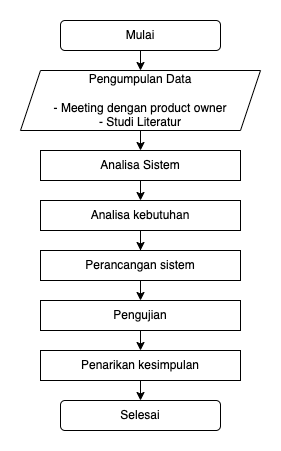
\includegraphics[width=0.4\textwidth]{gambar/tahapanpenelitian}
	\caption{Tahapan Peneltian}
	\label{fig:tahapan_penelitian}
\end{figure}


\section{Pengumpulan Data}

Data diambil dari hasil wawancara dengan owner J Farm Technology (JFT) Muhammad Eka Suryana, M.Kom., yang sekaligus merupakan klien dari penelitian ini. Selain itu, dilakukan studi literatur dengan membaca jurnal-jurnal yang terkait dengan topik penelitian. Setelah melakukan wawancara disimpulkan owner JFT membutuhkan suatu sistem web service untuk pengolahan data yang akan menerima request dari aplikasi mobile. Web service tersebut harus memiliki beberapa fitur diantaranya adalah pencatatan pemberian pakan setiap kolam, adanya fitur untuk meregistrasi kolam termasuk detail kolamnya, fitur untuk pencatatan masa budidaya pada setiap kolam termasuk dengan ikannya, fitur pencatatan kualitas air harian dan mingguan, pencatatan data kematian ikan, pencatatan treatment kolam, grading berat ikan kolam, perpindahan ikan antar kolam. Untuk transkrip wawancara dapat dibaca pada Lampiran 1.

\section{Analisa Sistem}

Sistem yang akan dihasilkan oleh penelitian ini berupa sebuah web service, lebih tepatnya adalah Private API. Sistem akan menggunakan arsitektur REST yang mana sering juga disebut RESTful. Sistem akan memberikan respons dari setiap request yang dilakukan oleh client. Request yang dilakukan oleh client memakai protokol http dan response yang diberikan oleh sistem berupa JSON Object. Yang nantinya sistem akan dijalankan di online server agar bisa di akses oleh client menggunakan akses internet.

\begin{figure}[H]
	\centering
	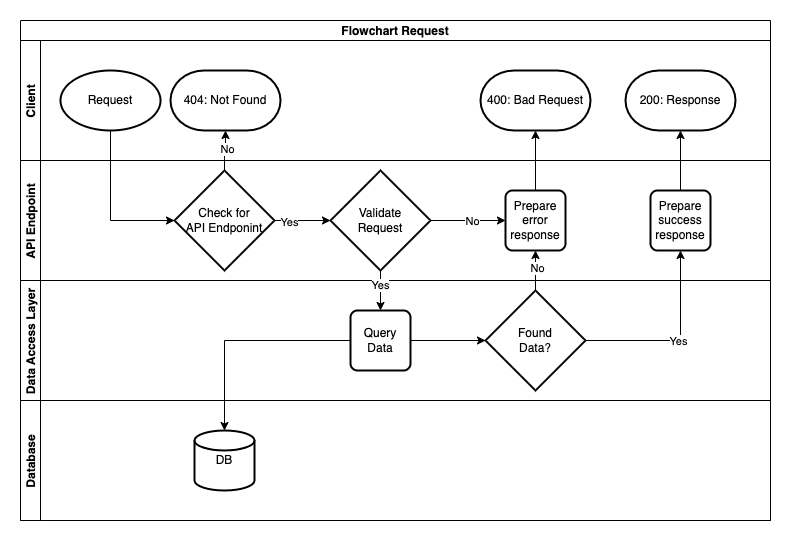
\includegraphics[width=0.85\textwidth]{gambar/flowchart_request_api.png}
	\caption{\emph{Flowchart} request}
	\label{fig:flowchart_request}
\end{figure}

Dimulai dari request yang dilakukan oleh client, ada beberapa proses yang akan dilakukan oleh sistem. Proses yang dilakukan oleh sistem diantaranya adalah pengecekan API EndPoint, validasi request, pengambilan dan penulisan data di database, dan persiapan response. Pengecekan API EndPoint dilakukan oleh sistem untuk mengetahui request apa yang diminta oleh client dari URL yang diakses. validasi request dilakukan untuk memastikan data yang dikirim oleh user telah sesuai dengan protokol yang telah ditentukan. Setelahnya proses yang dilakukan adalah memanipulasi atau membaca data di database. dan diakhiri dengan persiapan protokol response sebelum dikirim ke client.

\begin{figure}[H]
	\centering
	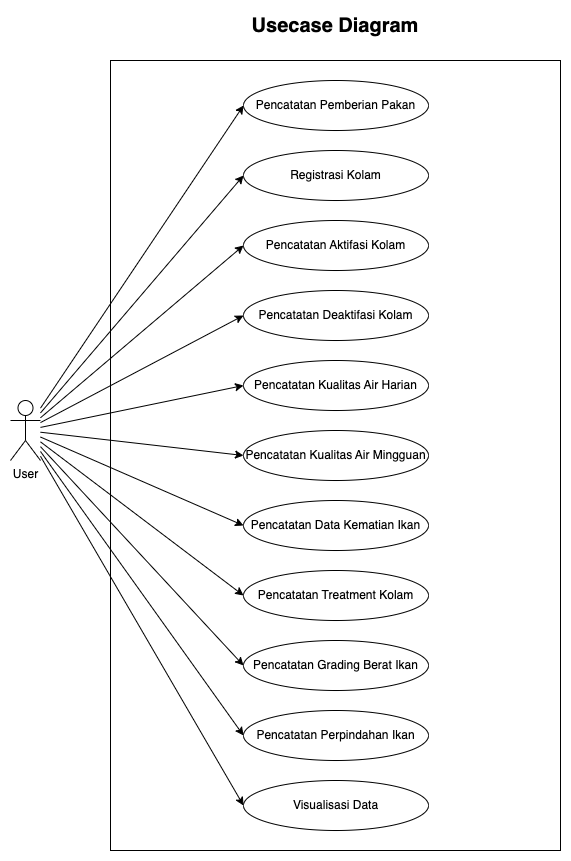
\includegraphics[height=0.9\textwidth]{gambar/usecase_diagram.png}
	\caption{\emph{Usecase} diagram}
	\label{fig:usecase_diagram}
\end{figure}

\textbf{Gambar \ref{fig:usecase_diagram}} merupakan usecase diagram user yang dibuat berdasarkan story yang telah didiskusikan bersama \textit{scrum master}. usecase tersebut menggambarkan kegiatan apa saja yang bisa dilakukan oleh user dalam menggunakan aplikasi. Pada penerapan pada \textit{backend usecase} nantinya akan di pecah lebih mendetail saat mendeskripsikan \textit{task} dari \textit{story}.

\section{Analisa Kebutuhan}

Berdasarkan uraian pada lampiran 1., prioritas fitur pada webservice perikanan modern terfokus pada pencatatan aktifitas pembudidaya ikan seperti pemberian pakan, pencatatan kematian ikan, dll.

Perangkat keras dan perangkat lunak yang penulis butuhkan adalah sebagai berikut:

\begin{enumerate}
\item Perangkat keras, terdiri dari:
\begin{enumerate} [a.]
\item Laptop dengan spesifikasi Processor Apple M1 \& Ram 8 GB
\end{enumerate}
\item Perangkat lunak, terdiri atas:
\begin{enumerate} [a.]
\item MacOs ventura 13.0
\item Visual Studio Code sebagai IDE dan code editor
\item Python sebagai bahasa pemrograman penyusun aplikasi web service
\item Flask sebagai framework python
\item MongoDB sebagai basis data
\end{enumerate}
\end{enumerate}

\section{Perancangan Sistem}

Untuk keberlangsungan penelitian, penulis menggunakan metodologi pengembangan sistem scrum Adapun tahapan-tahapan bagian dari scrum yang dilakukan dalam proses penelitian skripsi yang berjudul “Perancangan Arsitektur Backend Server Teknologi Perikanan Modren Berikut Spesifikasi Web Service yang Mampu Berhubungan dengan Multi Platform dengan Metode Scrum”. Flowchart metodologi Scrum yang dapat dilihat pada \textbf{Gambar \ref{fig:flowchart_scrum}}.

\begin{figure}[H]
	\centering
	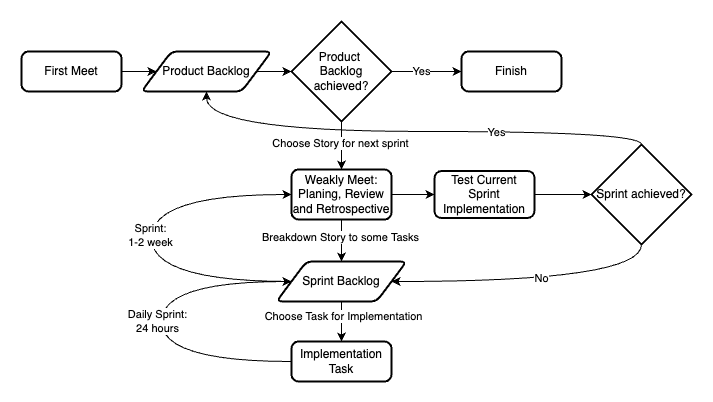
\includegraphics[height=0.6\textwidth]{gambar/design_penelitian_revisi.png}
	\caption{Flowchart Scrum}
	\label{fig:flowchart_scrum}
\end{figure}

Tahapan pertama penelitian adalah melakukan meeting dengan product owner dan scrum master. Meeting tersebut bertujuan untuk mendefinisikan product backlog yang akan menjadi acuan sprint kedepannya. Berikutnya merupakan weekly meeting pertama, agenda pada meeting ini adalah sprint planning. Sprint planning dilakukan dengan cara memilih story dari product backlog yang akan dilakukan breakdown sehingga menghasilkan sprint backlog. Sprint backlog merupakan kumpulan dari task-task kecil yang akan diimplementasi oleh developer setiap harinya. Weekly meeting berikutnya memiliki agenda tambahan dibanding dengan weekly meeting pertama yaitu, adanya sprint review dan sprint retrospective sebelum dilakukannya sprint planning untuk minggu berikutnya. Sprint review dan retrospective merupakan sebuah kajian dari task yang sudah dikerjakan oleh developer dan sprint yang dilakukan bersama oleh scrum master. Apabila tujuan dari sprint itu tercapai, maka scrum master akan menentukan story dari product backlog untuk sprint selanjutnya. Setelah semua product backlog tercapai maka sistem bisa dikatakan telah selesai.

Metode scrum terdiri dari beberapa komponen diantaranya adalah product backlog, sprint backlog, sprint, daily scrum, dan pengujian sistem. Berikut adalah penjelasan dari komponen-komponen tersebut:

	\subsection{Produk Backlog}
	
	Product backlog dibuat berdasarkan hasil diskusi dengan product owner sekaligus scrum master. Transkrip percakapan diskusi terdapat pada \textbf{Lampiran}. Setiap story yang ada di product backlog akan diselesaikan bertahap tiap minggunya. Berikut adalah tabel product backlog.
	
\begin{table}[H]
	\centering
	\caption{\textit{Product Backlog}}
	\label{table:product_backlog}
	\begin{tabular}{@{} |p{0.5cm}|p{10cm}|p{1cm}|p{2cm}| @{}}
		\hline
		\textbf{No} & \textbf{User Story} & \textbf{Sprint} & \textbf{Priority}\\
		\hline
		1 & Modul CRUD dan tampilan Pencatatan Pemberian pakan &  1,2 & High\\
		\hline
		2 & Modul CRUD dan tampilan untuk Registrasi kolam&  3 & High\\
		\hline
		3 & Modul CRUD dan tampilan untuk Masa Budidaya Kolam &  4 & High\\
		\hline
		4 & Modul CRUD dan tampilan untuk Pencatatan data kematian ikan &  5,6 & Medium\\
		\hline
		5 & Modul CRUD dan tampilan untuk Pencatatan Sortir ikan &  7 & Medium\\
		\hline
		6 & Modul CRUD dan tampilan untuk Pencatatan Grading berat ikan &  8 & Medium\\
		\hline
		7 & Modul CRUD dan tampilan untuk Pencatatan kualitas air harian &  9 & Low\\
		\hline
		8 & Modul CRUD dan tampilan untuk Pencatatan kualitas air mingguan &  9 & Low\\
		\hline
		9 & Modul CRUD dan tampilan untuk Pencatatan treatment kolam &  10 & Low\\
		\hline
	\end{tabular}
\end{table}
	
	Dari \textbf{Tabel \ref{table:product_backlog}} di atas, Produk Backlog terdiri dari empat komponen yaitu, User Story, Sprint, dan Priority. Story merupakan sebuah pekerjaan yang menggambarkan suatu fitur atau suatu module, yang mana nantinya akan diuraikan kedalam sprint dalam bentuk task. Komponen sprint merupakan perkiraan pada sprint keberapakah story akan dikerjakan. Priority merupakan sebuah keterangan seberapa prioritasnya user story.
	
	\subsection{Sprint Backlog}
	
	Sprint backlog merupakan sebuah task atau pekerjaan yang cenderung lebih kecil atau ringan. Sprint backlog merupakan uraian dari satu story pada product backlog yang menghasilkan beberapa task ringan. Sprint backlog diuraikan oleh scrum master. kemudian, developer bisa memilih task mana yang akan dikerjakan dahulu. Berikut merupakan tabel sprint backlog pertama.
	
	\begin{enumerate}
	
		\item Sprint-1
		
		Sprint-1 dilaksanakan selama delapan minggu yaitu pada tanggal 5 April sampai 31 Mei 2021. delapan minggu tersebut dikarenakan terdapatnya libur lebaran idul fitri selama 2 minggu yaitu pada tanggal 25 April - 9 May. Lalu enam minggu sisanya merupakan waktu yang dibutuhkan penulis untuk menulis penelitian, pembelajaran Scrum, pembelajaran framework flask, dan pembelajaran deployment pada server. Sprint ini merupakan uraian dari story "Pencatatan pemberian pakan" pada product backlog.
		
	\end{enumerate}
	
	\begin{table}[H]
	\caption{\textit{Sprint-1 backlog}}
	\label{sprint1_backlog}
	\begin{tabular}{@{} |p{0.5cm}|p{5cm}|p{5cm}|p{2cm}| @{}}
		\hline
		\textbf{No} & \textbf{\textit{Story}} & \textbf{\textit{Task}} & \textbf{\textit{Status}} \\
		\hline
		1 & \multirow{10}{5cm}{Create, Read, Updte, dan Delete untuk Pencatatan Pemberian pakan} & Merancang Database & Completed\\
		\cline{1-1}\cline{3-4}
		2 & & Merancang struktur flask framework & Completed\\
		\cline{1-1}\cline{3-4}
		3 & & Merancang class diagram & Completed\\
		\cline{1-1}\cline{3-4}
		4 & & Implementasi model Pond, Feed\_type, Feed\_history & Tested\\
		\cline{1-1}\cline{3-4}
		5 & & Implementasi controller EndpointApi & Tested\\
		\cline{1-1}\cline{3-4}
		6 & & Deployment Sistem & Tested\\
		\cline{1-1}\cline{3-4}
		7 & & Konfigurasi sistem di server & Tested\\
		\cline{1-1}\cline{3-4}
		8 & & Merancang Dokumentasi API & Tested\\
		\hline
	\end{tabular}
	\end{table}
	
	\subsection{Daily Scrum}
	
	Daily scrum tidak dilakukan secara meeting dikarenakan terbatasnya waktu scrum master dan developer. Maka dari itu, daily scrum digantikan dengan mencatat hambatan dan hal penting yang terjadi pada saat menjalankan sprint setiap harinya pada note github projects.
	
	\subsection{Sprint Review dan Sprint Retrospective}
	
	Sprint review dan retrospective dilakukan pada awal pekan tepatnya pada hari selasa. Sprint review dan retrospective dilakukan dengan cara voice call melalui platform telegram dan discord. Pembahasan dari meeting ini dimulai dari evaluasi perkembangan sistem, hambatan yang terjadi, dan penetapan sprint kedepannya.
		
\section{Pengujian}
Pada tahap ini peneliti akan melakukan uji backend server perikanan modern menggunakan dua jenis pengujian yaitu unit testing dan User Acceptance Test (UAT). Pengujian unit testing dilaksanakan oleh developer untuk memastikan fungsi-fungsi pada aplikasi yang telah dikembangkan dapat berjalan dengan baik. Sedangkan UAT dilaksanakan oleh scrum master untuk mengetahui apakah backend server sudah sesuai dengan kebutuhan dan layak untuk dipakai oleh developer frontend.

\begin{enumerate}
\item Unit Testing
Skenario pada unit testing dibuat berdasarkan skenario pemakaian web service yang ada pada fitur-fitur di product backlog. Skenario pemakaian web service adalah dengan melakukan request terhadap endpoint api yang ada pada setiap fitur. Setiap fitur setidaknya memiliki 4 skenario request yaitu GET, POST, PUT, DELETE. Adapun skenario dari unit testing yang akan diuji oleh developer terdapat pada \textbf{Tabel \ref{table:unit_testing}}.
\begin{longtable}{| p{3cm} | p{10cm} |}
\caption{Skenario unit testing.\label{table:unit_testing}}\\

\hline
\multicolumn{2}{| c |}{Awal Tabel}\\
\hline
\multicolumn{1}{|c|}{\textbf{Uji unit}} & \multicolumn{1}{|c|}{\textbf{Skenario Pengujian}}\\
\hline
\endfirsthead

\hline
\multicolumn{2}{|c|}{Lanjutan \textbf{Tabel \ref{table:unit_testing}}}\\
\hline
\multicolumn{1}{|c|}{\textbf{Uji unit}} & \multicolumn{1}{|c|}{\textbf{Skenario Pengujian}}\\
\hline
\endhead

\hline
\endfoot

\hline
\multicolumn{2}{|c|}{Akhir \textbf{Tabel \ref{table:unit_testing}}}\\
\hline\hline
\endlastfoot

Pemberian Pakan                  & Request POST API pencatatan pemberian pakan                                                    \\ \cline{2-2}
                                 & Request PUT API merubah data pemberian pakan                                              \\ \cline{2-2}
                                 & Request GET API mendapatkan list data pemberian pakan pada suatu kolam                                      \\ \cline{2-2}
                                 & Request GET API mendapatkan detail data pemberian pakan                                     \\ \cline{2-2}
                                 & Request DELETE API hapus data pemeberian pakan                                                  \\ \hline
Registrasi Kolam                 & Request POST API pencatatan registasi kolam                                                   \\ \cline{2-2}
                                 & Request PUT API merubah data kolam                                                           \\ \cline{2-2}
                                 & Request GET API mendapatkan list data kolam                                                  \\ \cline{2-2}
                                 & Request GET API mendapatkan detail data kolam                                                \\ \cline{2-2}
                                 & Request DELETE API hapus data kolam                                                             \\ \hline
Musim Budidaya Kolam            & Request POST API memulai musim budidaya pada kolam                                            \\ \cline{2-2}
                                 & Request POST API mengakhiri musim budidaya atau panen pada kolam                              \\ \cline{2-2}
                                 & Request GET API mendapatkan list musim budidaya pada suatu kolam                             \\ \hline
Pencatatan Kematian Ikan         & Request POST API pencatatan kematian ikan                                                     \\ \cline{2-2}
                                 & Request PUT API merubah data kematian ikan                                                   \\ \cline{2-2}
                                 & Request GET API mendapatkan list data kematian ikan pada suatu musim budidaya                \\ \cline{2-2}
                                 & Request GET API mendapatkan detail kematian ikan                                             \\ \cline{2-2}
                                 & Request DELETE API hapus kematian ikan                                                          \\ \hline
Perpindahan Ikan Antar Kolam     & Request POST API pencatatan perpindahan ikan antar kolam                                      \\ \cline{2-2}
                                 & Request PUT API merubah data perpindahan ikan antar kolam                                    \\ \cline{2-2}
                                 & Request GET API mendapatkan list data perpindahan ikan pada suatu musim budidaya             \\ \cline{2-2}
                                 & Request GET API mendapatkan detail perpindahan ikan                                          \\ \cline{2-2}
                                 & Request DELETE API hapus data perpindahan ikan                                                  \\ \hline
Grading berat ikan               & Request POST API pencatatan grading berat ikan                                                \\ \cline{2-2}
                                 & Request PUT API merubah data grading berat ikan                                              \\ \cline{2-2}
                                 & Request GET API mendapatkan list data grading berat ikan pada suatu musim budidaya           \\ \cline{2-2}
                                 & Request GET API mendapatkan detail grading berat ikan                                        \\ \cline{2-2}
                                 & Request DELETE API hapus data grading berat ikan                                                \\ \hline
Pencatatan kualitas air harian   & Request POST API pencatatan kualitas air harian kolam                                         \\ \cline{2-2}
                                 & Request PUT API merubah data kualitas air harian kolam                                       \\ \cline{2-2}
                                 & Request GET API mendapatkan list data kualitas air harian kolam pada suatu musim budidaya    \\ \cline{2-2}
                                 & Request GET API mendapatkan detail kualitas air harian                                 \\ \cline{2-2}
                                 & Request DELETE API hapus data kualitas air harian kolam                                         \\ \hline
Request POST Pencatatan kualitas air mingguan & API pencatatan kualitas air mingguan kolam                                       \\ \cline{2-2}
                                 & Request PUTAPI merubah data kualitas air mingguan kolam                                     \\ \cline{2-2}
                                 & Request GET API mendapatkan list data kualitas air mingguan kolam pada suatu musim budidaya  \\ \cline{2-2}
                                 & Request GET API mendapatkan detail kualitas air mingguan kolam                               \\ \cline{2-2}
                                 & Request DELETE API hapus data kualitas air mingguan kolam                                       \\ \hline
Pencatatan treatment kolam & Request POST API pencatatan treatment kolam                                       \\ \cline{2-2}
                                 & Request PUT API merubah data treatment kolam                                     \\ \cline{2-2}
                                 & Request GET API mendapatkan list data treatment kolam pada suatu musim budidaya  \\ \cline{2-2}
                                 & Request GET API mendapatkan detail treatment kolam                               \\ \cline{2-2}
                                 & Request DELETE API hapus data treatment kolam                                       \\ \hline
\end{longtable}
\item User Acceptance Test
Skenario pada User Acceptance Test dibuat berdasarkan fitur-fitur yang dapat diakses oleh owner. Fitur yang digunakan oleh owner adalah dashboard admin table yang menampilkan data-data yang telah di masukan ke dalam database. Adapun skenario dari UAT yang akan dilaksanakan terdapat pada tabel

\begin{longtable}{| p{8cm} | c | c | l |}
\caption{Daftar pengujian UAT.\label{table:skenario_uat}}\\
\hline
\multicolumn{4}{| c |}{Awal Tabel}\\
\hline
\multirow{2}{*}{Skenario Pengujian UAT} & \multicolumn{2}{l|}{Kesesuaian}            & \multirow{2}{*}{Kesimpulan} \\ \cline{2-3}
                                    & \multicolumn{1}{l|}{sesuai} & belum &                             \\ \hline
\hline
\endfirsthead
\hline
\multicolumn{4}{|c|}{Lanjutan \textbf{Tabel \ref{table:skenario_uat}}}\\
\hline
\multirow{2}{*}{Skenario Pengujian} & \multicolumn{2}{l|}{Kesesuaian}            & \multirow{2}{*}{Kesimpulan} \\ \cline{2-3}
                                    & \multicolumn{1}{l|}{sesuai} & belum &                             \\ \hline
\hline
\endhead
\hline
\endfoot
\hline
\multicolumn{4}{|c|}{Akhir \textbf{Tabel \ref{table:skenario_uat}}}\\
\hline\hline
\endlastfoot
Menampilkan dashboard tabel ketika mengakses http://jft.web.id/fishapi/ & & & \\ \hline
Tampilan tabel pencatatan pemberian pakan keseluruhan ketika mengeklik pencatatan pemberikan pakan pada sidebar dashboard &&&\\ \hline
Tampilan tabel pencatatan pemberian pakan harian ketika mengeklik pencatatan pemberikan pakan harian pada sidebar dashboard &&&\\ \hline
Tampilan tabel pencatatan pemberian pakan bulanan ketika mengeklik pencatatan pemberikan pakan bulanan pada sidebar dashboard &&&\\ \hline
Tampilan tabel kolam yang sudah di registrasi ketika mengkelik kolam -> detail pada sidebar dashboard&&&\\ \hline
Tampilan tabel masa budidaya kolam ketika mengkelik kolam -> masa budidaya pada sidebar dashboard &&&\\ \hline
Tampilan tabel jumlah Ikan setiap kolam ketika mengkelik kolam -> jumlah ikan pada sidebar dashboard &&&\\ \hline
Tampilan tabel data kematian ikan ketika mengkelik kematian ikan pada sidebar dashboard &&&\\ \hline
Tampilan tabel data sortir ikan ketika mengkelik sortir ikan pada sidebar dashboard &&&\\ \hline
Tampilan tabel data grading berat ikan ketika mengkelik grading ikan pada sidebar dashboard &&&\\ \hline
Tampilan tabel data kualitas air harian ketika mengkelik kualitas air -> harian pada sidebar dashboard &&&\\ \hline
Tampilan tabel data kualitas air mingguan ketika mengkelik kualitas air -> mingguan pada sidebar dashboard &&&\\ \hline
Tampilan tabel data treatment kolam ketika mengkelik treatment kolam pada sidebar dashboard &&&\\ \hline
\end{longtable}

\end{enumerate}
	

	
% Baris ini digunakan untuk membantu dalam melakukan sitasi
% Karena diapit dengan comment, maka baris ini akan diabaikan
% oleh compiler LaTeX.
\begin{comment}
\bibliography{daftar-pustaka}
\end{comment}